\section{Experiments}
\label{sec5}
We present our experimental results in this section. In Section \ref{sec5-1}, we introduce the datasets and metrics used in the evaluation. We comprehensively validate our model through zero-shot benchmarks in both English and Chinese in Section \ref{sec5-2}.
%We consider both bilingual and monolingual scenarios, to comprehensively validate the language capabilities, through zero-shot performances. We then present the general performances on the selected benchmarks to compare AltCLIP and the state-of-the-art image-text models. 
In Section \ref{sec5-3}, we conduct an ablation study on the effects of various design choices in Teacher Learning and Contrastive Learning. 
Finally, in Section \ref{sec5-4}, we use an AltCLIP-guided diffusion model to generate images from both Chinese and English prompts, and show that our model is capable to align text in different languages.
%In addition, examples of generated images from bilingual text prompts through AltCLIP-guided diffusion model are shown to ``visualize" the language capabilities.

%As mentioned above, we perform evaluations on both bilingual and monolingual benchmarks. 

%Bilingual benchmarks require image collections with associated parallel bilingual texts.
%\ledell{Here we should say ImageNet is an important benchmark for evaluating Vision pretraining model, instead of 'we have the translation'}
\subsection{Evaluation Datasets and Metrics} 
\label{sec5-1}
In this section, we describe the datasets and metrics we used in our experiments. We use ImageNet ~\cite{deng2009imagenet} and its four out-of-distribution test variants, i.e. ImageNet Sketch~\cite{wang2019learning}, ImageNet-A~\cite{hendrycks2021natural}, ImageNet-R~\cite{hendrycks2021many}, ImageNetV2~\cite{recht2019imagenet}, to evaluate zero-shot image classification performances in English and Chinese. \footnote{We use the Chinese translation of classnames from \url{https://github.com/ningbonb/imagenet_classes_chinese}}
%ImageNet is widely-applied to assess consistent performances on natural distributions for vision pretraining models.
During evaluation, we adapt the templates of manual prompts from CLIP for English and corresponding machine translation templates for Chinese. For cross-modal retrieval, we select Flickr30k~\cite{young2014image}, MSCOCO~\cite{lin2014microsoft}, as well as their corresponding Chinese datasets, Flickr30k$_\text{CN}$~\cite{lan2017fluency}, MSCOCO$_\text{CN}$~ \footnote{two versions, texts in 1k version are manual written captions while in 5k version are manual translated captions}~\cite{li2019coco}, to evaluate zero-shot image-to-text retrieval and text-to-image retrieval performances. 

We further validate our model on a wide range of tasks to compare the performance with the original CLIP model. We collect the datasets introduced in CLIP and the Open CLIP benchmark \footnote{\url{https://github.com/LAION-AI/CLIP_benchmark}}, including Birdsnap~\cite{berg2014birdsnap}, Caltech-101~\cite{fei2006one}, Stanford Cars~\cite{Krause2013}, CIFAR-10~\cite{krizhevsky2009learning}, CIFAR-100~\cite{krizhevsky2009learning}, Country211~\cite{radford2021learning}, DTD~\cite{cimpoi2014describing}, EuroSAT~\cite{helber2019eurosat}, Facial Emotion Recognition 2013~\cite{goodfellow2013challenges}, FGVC Aircraft~\cite{blaschko2012towards}, Oxford Flowers 102~\cite{nilsback2008automated}, Food-101~\cite{bossard14}, GTSRB~\cite{stallkamp2011german}, Kinetics400~\cite{kay2017kinetics}, Kinetics600~\cite{carreira2018short}, MNIST~\cite{cirecsan2011high}, PatchCamelyon~\cite{veeling2018rotation}, ObjectNet~\cite{barbu2019objectnet}, Oxford-IIIT Pets~\cite{parkhi2012cats}, Rendered SST2~\cite{radford2021learning}, RESISC45~\cite{cheng2017remote}, STL-10~\cite{coates2011analysis}, SUN397~\cite{Xiao2010}, UCF101~\cite{soomro2012ucf101}, Pascal VOC 2007 Classification~\cite{pascal-voc-2007}, Pascal VOC 2007 Multilabel Classification~\cite{pascal-voc-2007}. 
%Additionally, more monolingual benchmarks are introduced in order to compare the performance on wider distributions and tasks with CLIP. 
%These datasets are collected from the well-studied evaluation introduced in CLIP ~\cite{radford2021learning} and the Open CLIP benchmark\footnote{\url{https://github.com/LAION-AI/CLIP_benchmark}}, an open-source project to evaluate Language-Image pretraining models, including Birdsnap, Caltech-101, Stanford Cars, CIFAR-10, CIFAR-100, Country211, DTD, EuroSAT, Facial Emotion Recognition 2013, FGVC Aircraft, Oxford Flowers 102, Food-101, GTSRB, Kinetics400, Kinetics600, MNIST, PatchCamelyon, Oxford-IIIT Pets, Rendered SST2, RESISC45, STL-10, SUN397, UCF101, Pascal VOC 2007 Classification, Pascal VOC 2007 Multilabel Classification. 
Finally, we evaluate our multilingual model AltCLIP$_{M9}$ on the \textbf{XTD} ~\cite{aggarwal2020zeroshot} dataset. XTD selected 1K images from MS COCO, and translated the corresponding English Captions into 11 languages (English(en), German(de), French(fr), Chinese(zh), Japanese(ja), Italian(it), Spanish(es), Russian(ru), Polish(pl), Turkish(tr), Korean(ko)).
The evaluation metrics for image classification benchmarks are respectively accuracy (default), mean per class (the average of recall obtained on each class, for imbalanced datasets, i.e. FGVC Aircraft, Oxford-IIIT Pets, Caltech-101, Oxford Flowers 102), 11-point mAP (mean average of 11-pt interpolated precision for each class, for VOC 2007), mean(top1, top5) (the mean of acc@1 and acc@5, for Kinetics400 and Kinetics600), while for cross-modal retrieval benchmarks, are Recall@K where $K\in\{1,5,10\}$, and Mean Recall(MR, i.e., the average of
Recall@K) for both image-to-text retrieval and text-to-image retrieval tasks, which are same with the setups in CLIP ~\cite{radford2021learning}.



\begin{table*}[t]
\centering
\small
\begin{tabular}{ccccccccc} 
\hline
\diagbox{Method}{Language} & En            & Es            & Fr            & Zh            & It            & Ko            & Ru            & Jp             \\ 
\hline
CLIP$_{ViT-B32}$                       & 90.3          & -             & -             & -             & -             & -             & -             & -              \\
CLIP$_{ViT-L14}$                       & 91.8          & -             & -             & -             & -             & -             & -             & -              \\
CLIP$_{ViT-B16+}$$\dag$                       & 94.3          & -             & -             & -             & -             & -             & -             & -              \\
mUSE PATR                      &83.6  &75.6 &76.9 &76.1 &73.4 &64.3 &73.6  &69.4            \\
mUSE m3             &85.3  &78.9 &78.9 &76.7 &73.6 &67.8 &76.1  &70.7         \\
M-CLIP$_{ViT-B32}$                     &91.8		&89.1	&89.4	&89.3	&89.8		&82.1	&86.1		&81.0           \\
M-CLIP$_{ViT-L14}$                     & 92.4          & 91            & 90            & 89.7          & 91.1          & 85.2          & 85.8          & 81.9           \\
M-CLIP$_{ViT-B16+}$$\dag$      &95   &93.6	&\textbf{93.1}	&94	&93.1		&89	&90	&84.2      \\
%AltCLIP$^T_{M9}$                & 94.7          & 91.2          & 91.3          & 93.7          & 92.9          & 92.7          & 89.9          & 89.8           \\
AltCLIP$_{M9}$                    & \textbf{95.4} & \textbf{94.1} & 92.9 & \textbf{95.1} & \textbf{94.2} & \textbf{94.4} & \textbf{91.8} & \textbf{91.7}  \\
\hline
\end{tabular}
\caption{Comparison results on the multilingual cross-modal Retrieve dataset XTD.  Following M-CLIP, we report recall@10 on Image to Text. \dag  represents using image encoder released by OpenCLIP project ~\cite{ilharco_gabriel_2021_5143773}. 
%We report all result from official report. 
\label{tab:xtd}}
\end{table*}
% \begin{table*}[tb]
% \small
% \centering
% \begin{tabular}{ccccccc}\hline
% EN-EN & EN-CN & Both & Flickr30k$_{EN}$ & Flickr30k$_{CN}$ & ImageNet$_{EN}$ & ImageNet$_{CN}$ \\\hline
% %CN-Our-xmlr  & Laion28m          &                   &                            & 87.01        & 5.5          & 70.3        & 2           \\
%  \Checkmark             &                   &                              & 86.59        & 53.86        & 53.76       & 12.84       \\
%                      & \Checkmark             &                              & 61.89        & 85.37        & 15.47       & 42.47       \\
% % \Checkmark             & \Checkmark              &                              & 79.82        & 85.60         & 32.77       & 42.20        \\
%                      &                     & \Checkmark                   & 86.82        & 85.84        & 51.61       & 41.66       \\\hline
% %CN-Ours-xmlr &                   &                   & Laion28M                   & 87.76        & 86.05        & 73.85       & 46.21      \\\hline
% \end{tabular}
% \caption{Ablation Experiments on parallel text used in Teacher Learning. En-En indicates the use of English-English text pairs; En-Cn indicates the use of English-Chinese parallel text. \label{tab:pkd}}
% \end{table*}
% \usepackage{booktabs}


\begin{table*}[tb]
\centering
\small
\begin{tabular}{cccc|cccc} 
\toprule
EN-EN & EN-CN$_{MT}$ & EN-CN$_{HT}$ & CL             & \multicolumn{1}{l}{Flickr30K$_{EN}$} & \multicolumn{1}{l}{Flickr30K$_{CN}$} & \multicolumn{1}{l}{ImageNet$_{EN}$} & \multicolumn{1}{l}{ImageNet$_{CN}$}  \\ 
\midrule
\Checkmark                &\Checkmark&\Checkmark&\Checkmark& \textbf{90.4}                                 & \textbf{89.2}                                   & 74.5                                & \textbf{59.6}                           \\

\Checkmark             &\Checkmark&\Checkmark&& 88.3                                 & 87.2                                   & \textbf{74.7}                                & 58.2                                 \\

\Checkmark &\Checkmark&&& 86.8                                & 85.8                                  & 51.6                               & 41.7                                \\

\Checkmark  &&&& 86.6                                & 53.9                                  & 53.8                               & 12.8                                \\

   &\Checkmark&&& 61.9                               & 85.4                                  & 15.5                               & 42.5                                \\
% \quad -w/ EN\&CN & 86.8                                & 85.8                                  & 51.6                               & 41.7                                \\
\bottomrule
\end{tabular}
\caption{Ablation Experiments. CL indicates the use of Contrastive Learning stage, while EN-EN, \text{EN-CN}$_{MT}$, \text{EN-CN}$_{HT}$ refers to parallel data used in Teacher Learning stage. Specifically, EN-EN indicates the use of English-English text pairs; EN-CN indicates the use of English-Chinese parallel text, including \text{EN-CN}$_{MT}$ represents machine translated pairs while \text{EN-CN}$_{HT}$ stands for human-translated data, i.e TSL2019. All compared models are pre-trained for 10 epochs. $\label{tab:pkd}$}
\end{table*}

% \begin{table*}[tb]
% \centering
% \begin{tabular}{l|cccc} 
% \toprule
% Methods             & \multicolumn{1}{l}{Flickr30K$_{EN}$} & \multicolumn{1}{l}{Flickr30K$_{CN}$} & \multicolumn{1}{l}{ImageNet$_{EN}$} & \multicolumn{1}{l}{ImageNet$_{CN}$}  \\ 
% \midrule
% Ours                & \textbf{90.4}                                 & \textbf{89.2}                                   & 74.5                                & \textbf{59.6}                           \\
% -w/o CL             & 88.3                                 & 87.2                                   & \textbf{74.7}                                & 58.2                                 \\
% -w/o CL\&Parallel Data & 86.8                                & 85.8                                  & 51.6                               & 41.7                                \\
% \quad -w/ EN-EN  & 86.6                                & 53.9                                  & 53.8                               & 12.8                                \\
% \quad -w/ EN-CN   & 61.9                               & 85.4                                  & 15.5                               & 42.5                                \\
% % \quad -w/ EN\&CN & 86.8                                & 85.8                                  & 51.6                               & 41.7                                \\
% \bottomrule
% \end{tabular}
% \caption{Ablation Experiments. CL indicates the use of Contrastive Learning and Parallel Data refers to human-translated data, i.e TSL2019. EN-EN indicates the use of English-English text pairs; EN-CN indicates the use of English-Chinese parallel text; EN\&CN indicates the use of English-Chinese parallel text and English-English parallel text. All compared models are pre-trained for 10 epochs. $\label{tab:pkd}$}
% \end{table*}


\subsection{Zero-shot performance}
\label{sec5-2}
%of AltCLIP with CLIP and CN-CLIP, which are respectively the previous sota English and Chinese CLIP-like model as far as we know.
%As illustrated in Table~\ref{tab:imagenet}, AltCLIP, regardless of after Teacher Learning process or contrastive learning process, achieve sota or nearly sota accuracy on both English and Chinese image classification benchmarks. On the contrary, the performances of  CLIP and CN-CLIP on the same image collections collapse, when switching the text to another language. Specifically, compared with CLIP, the average accuracy of AltCLIP on English datasets is only slightly lower, while on Chinese datasets, AltCLIP outperforms CLIP by a large margin, over 50.0 absolute average accuracy. Moreover, compared to CN-CLIP, on both languages, AltCLIP achieves better accuracy on almost all datasets, except the Chinese ImageNet Sketch Dataset. The statistics show both the extended Chinese language capabilities and consistent English language capabilities.
\paragraph{Image Classification}
We first present evaluation results of zero-shot image classification on the ImageNet dataset and its four out-of-distribution variants. For baselines, we compare our model with CLIP ~\cite{radford2021learning}, CN-CLIP ~\cite{yang2022chinese}, and multilingual CLIP (M-CLIP) ~\cite{carlsson2022cross}.
As illustrated in Table~\ref{tab:imagenet}, AltCLIP achieves results that are very close to CLIP in English and sets new state-of-the-art results on Chinese ImageNet, ImageNet-A, ImageNet-R, and ImageNet V2. These results demonstrate the effectiveness of our method: compared to other Chinese baseline models where hundreds of millions of text-image pairs are used in pretraining, we only use 36M parallel text data and 2M text-image pairs in training.

\paragraph{Cross-modal Retrieval}
For cross-modal retrieval, we compare our model with CLIP in English and R2D2 ~\cite{xie2022zero}, Wukong ~\cite{gu2022wukong}, Taiyi ~\cite{fengshenbang} and CN-CLIP ~\cite{yang2022chinese} in Chinese. The results are shown in Table~\ref{tab:retrieval}. AltCLIP outperforms all baseline models on most datasets and tasks. We notice that AltCLIP outperforms CLIP on both text-to-image and image-to-text retrieval. This could be due to the following reasons: 1). We used a small subset (less than 1M) of LAION 5B at the Contrastive Learning stage, which is in a different distribution of the pretraining data used in CLIP; 2). Our language encoder initialized from XLM-R provides better language understanding ability. We left it as a future investigation to properly analyze the factors.

%An interesting phenomenon is that on English datasets, AltCLIP outperforms CLIP on both text-to-image retrieval and image-to-text retrieval. This might indicate that the proposed approach, extends the language capabilities, by not only increasing the comprehension of target language, but also improving the matching abilities of image and source language.
\paragraph{Multilingual Cross-modal Retrieval}
%In order to evaluate the scalability of our method, we expanded the language to 8 languages, namely English(En), Chinese(Zh), Spanish(Es), French(Fr), Russian(Ru), Japanese(Ja), Korean(Ko), and Italian(It).
% Different from the above bilingual experiment, we translate LAION10M(subset of LAION400M) and CC3M and add 5M parallel corpus for each language. 
For baseline, we compare our model with CLIP, M-CLIP ~\cite{carlsson2022cross} and mUSE ~\cite{yang-etal-2020-multilingual}. The results of the comparison on XTD ~\cite{aggarwal2020zeroshot} are shown in Table \ref{tab:xtd}, where AltCLIP$_{M9}$ achieves state-of-the-art results in 7 languages. Notably, joint multilingual training maintains state-of-the-art capabilities in English and achieves better results than the original CLIP model on this dataset. We may achieve better results for two reasons: 1. We equally translate a fixed set of English captions for each language, which allows each language to share a more comprehensive distribution. 2. We introduce more parallel data of human translation, and experiments show that this part of the data is helpful for establishing a robust multilingual representation.
%demonstrating the linguistic scalability of our method.

\paragraph{Full CLIP benchmark}
We present the evaluation results of a wider range of tasks in English in Figure \ref{fig:clipbcm}. We compare the effectiveness of the Teacher Learning Stage and Contrastive Learning Stage, and the bilingual AltCLIP and multilingual AltCLIP$_{M9}$. We observe that at the Teacher Learning Stage, the model already learns a good representation of text-image representation, as it gets a close performance of the original CLIP model on a broad range of zero-shot benchmarks. The Contrastive Learning stage further improves our model’s performance, especially on retrieval tasks like Flickr30k and MSCOCO. Further, the multilingual AltCLIP$_{M9}$ achieves close performances with bilingual AltCLIP, indicating that our method is effective at extending the number of languages supported.

\subsection{Ablation study}
\label{sec5-3}
In this section, we present results from ablation studies. We show the significance of including various parallel data in Teacher Learning stage in Table \ref{tab:pkd}. As illustrated in the 3rd and 5th line, without English-to-English parallel data, the accuracy on English ImageNet drastically drops to 15.47 from 53.8. Similarly, excluding machine-translated English-to-Chinese data, has a great impact on the performances on Chinese benchmarks, i.e. Imagenet$_{CN}$ and Flickr30K$_{CN}$, due to influenced Chinese text-image representation. Moreover, empirical experiments show that introducing human translated parallel data leads to a great improvement on Imagenet$_{CN}$ which may be related to the distribution of the data set. This indicates that the diversity of training data used for teacher learning, can benefit the language model to gain more knowledge about entities or concepts.

%To evaluate our proposed two-stage training methods, we design several setups for the ablation study. Firstly, we evaluate the effects of our proposed distillation using XLM-R-base as student model. Secondly, we evaluate the effects of cross-lingual contrastive learning with the XLM-R-large model.
%\paragraph{Effects of parallel Teacher Learning}
%To effects of parallel Teacher Learning, we conduct a set of experiments under different parallel data settings.  As show in Tab.~\ref{tab:pkd}, the experimental results demonstrates that our proposed method can get a student model with well text-image alignment and cross-lingual abilities. 
%\paragraph{Effects of cross-lingual contrastive learning}
%To evaluate our proposed cross-lingual contrastive learning, we conduct a group of experiments with different contrastive learning settings. As show in Tab.~\ref{tab:ccl}, the cross-lingual contrastive learning help the model achieve significant higher performance on retrival tasks, e.g. Flickr30k and MSCOCO.

\subsection{Examples of text-to-image generation}
\label{sec5-4}
To demonstrate the effects of text alignment in our model, we use the text encoder of AltCLIP and AltCLIP$_{M9}$ to further finetune a text-to-image generation model from Stable Diffusion ~\cite{rombach2022high}.
We use stable-diffusion v1-4\footnote{https://huggingface.co/CompVis/stable-diffusion-v-1-4-original} as initialization, and we use AltCLIP or AltCLIP$_{M9}$ as the language encoder. We freeze all the parameters in the diffusion model except for the key and value projection layers of the cross-attention block during finetuning. The dataset we used to finetune is the same one used for Contrastive Learning as described in Section \ref{training data}. We call our image generation models AltDiffusion and AltDiffusion$_{M9}$. 

%We use the pre-trained bilingual language model as our text encoder and fine-tune it using the WuDao dataset (6M) with an aesthetic score above 5.5 and the Laion data (5M) with an aesthetic score above 5.5.

As shown in Fig.~\ref{fig:demo}, AltDiffusion generates high-quality images close to Stable Diffusion on both English and Chinese prompts. Further, we notice that our model generates very similar images given translated English and Chinese prompts. For the multilingual version, we observed a very interesting phenomenon: when given a prompt that’s translated into different languages, the generated images reflect cultural differences to some extent. See Tab. ~\ref{tab:m9} for some examples. We left it as a future effort to explore and analyze carefully on how culture inherited in different languages can affect image generation.

%As illustrated in Tab.~\ref{tab:m9}, our model generates images reflecting the culture in different languages. For example, Russian girls have very Russian-style head wears.

\begin{figure}
    \centering
    \subfigure[Stable Diffusion]{
    
\includegraphics[width=0.45\textwidth]{figures/1_sd.jpg}
    }
    \subfigure[AltDiffusion EN]{
    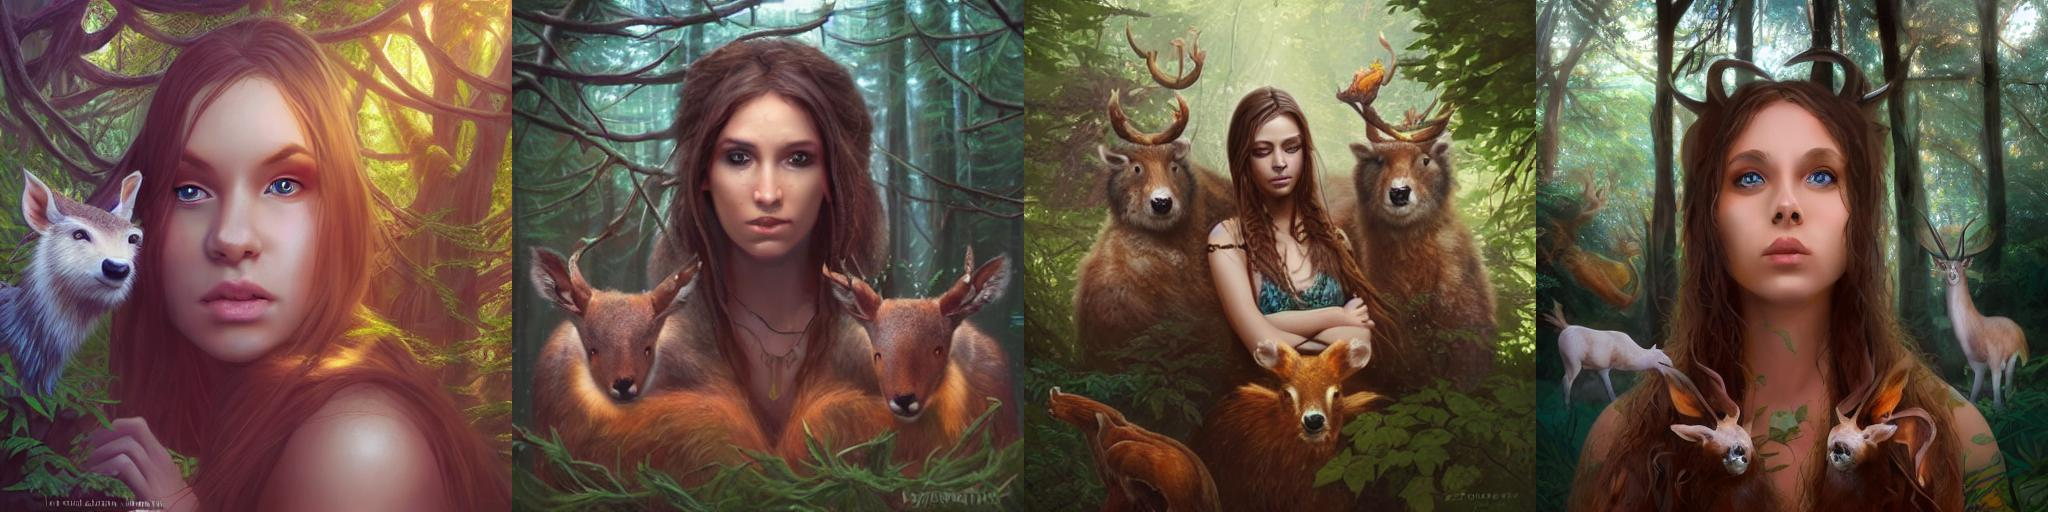
\includegraphics[width=0.45\textwidth]{figures/2_our.jpg}
    }
    \subfigure[AltDiffusion CN]{
    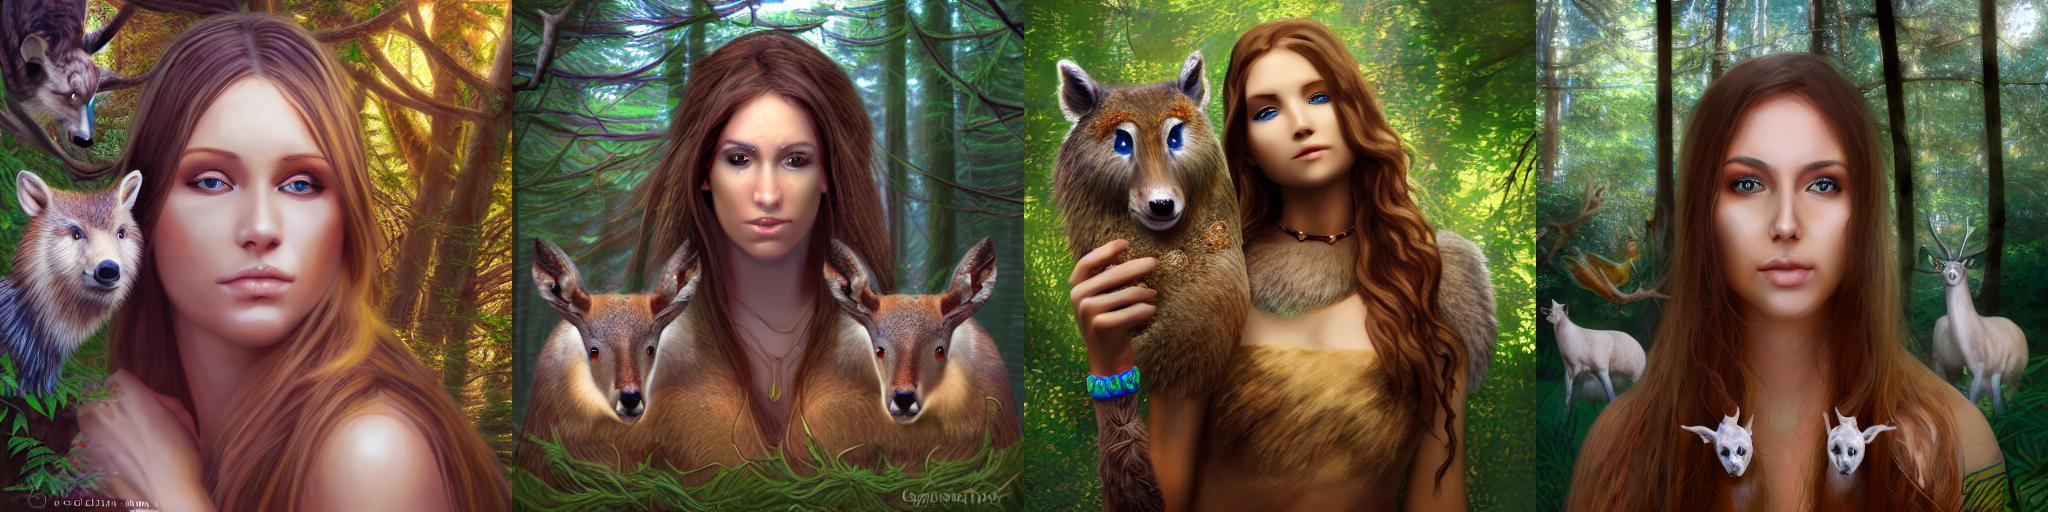
\includegraphics[width=0.45\textwidth]{figures/3_our_zh.jpg}
    }
    %\subfigure[An Open source bi-lingual Stable Diffusion EN]{
    %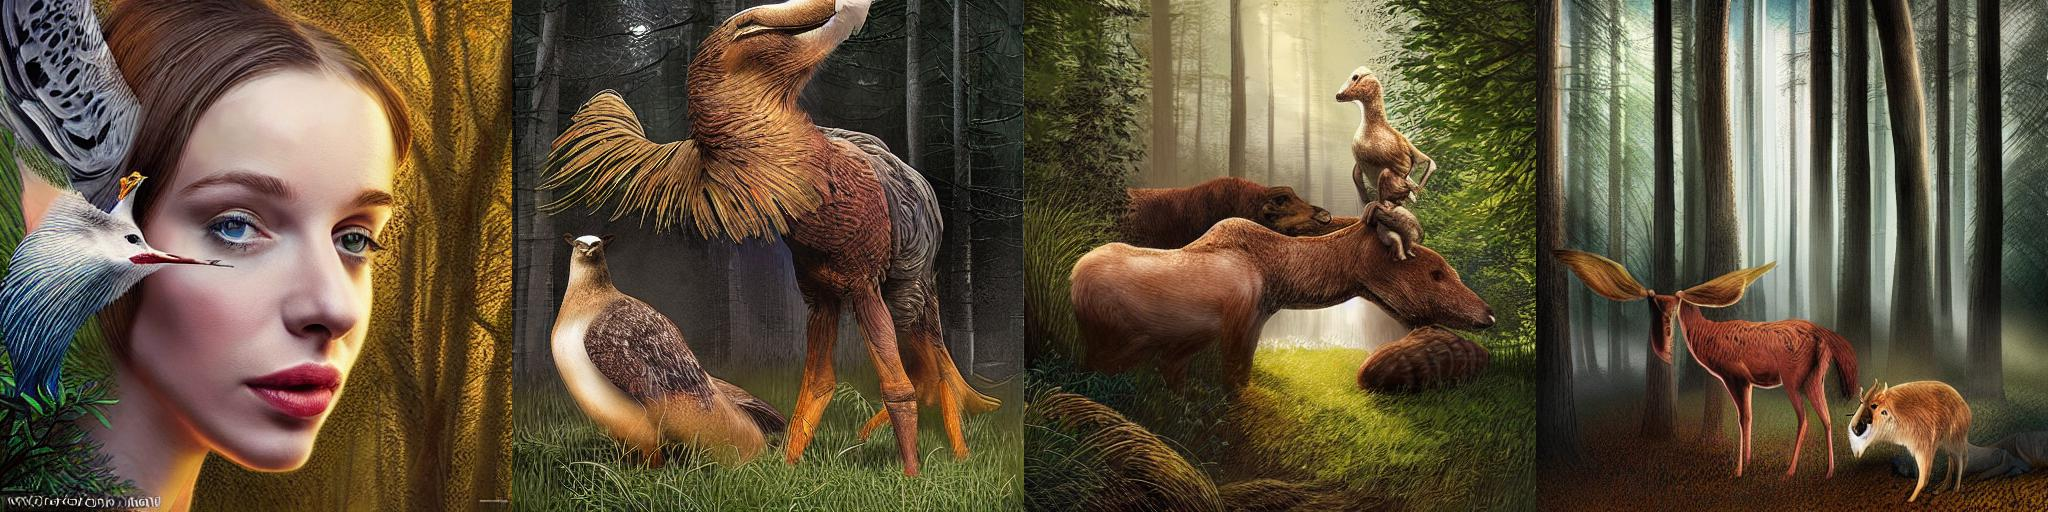
\includegraphics[width=0.45\textwidth]{figures/4_taiyi.jpg}
    %}
    %\subfigure[An Open source bi-lingual Stable Diffusion CN]{
    %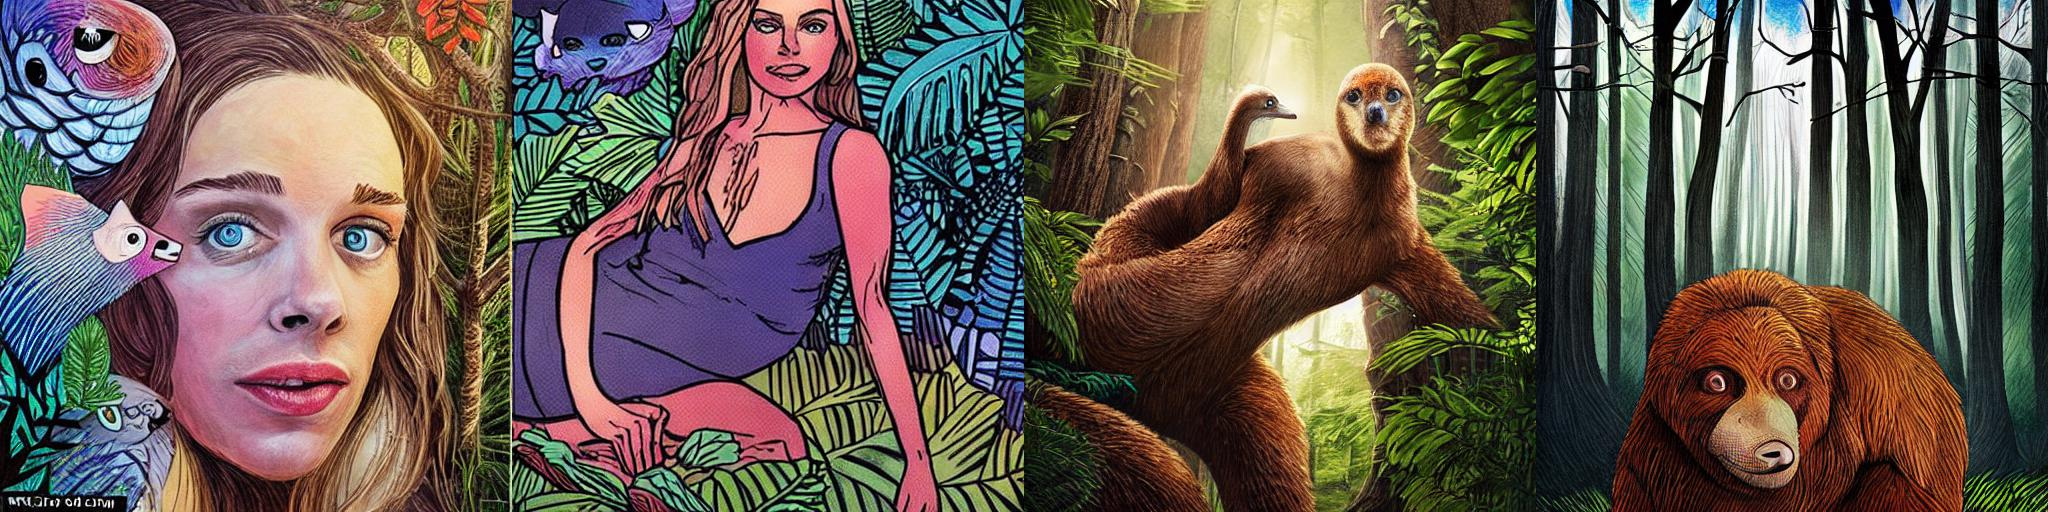
\includegraphics[width=0.45\textwidth]{figures/5_taiyi_zh.jpg}
    %}
    \caption{Examples of text-to-image generation. Text prompt: \textit{"a pretty female druid surrounded by forest animals, digital painting, photorealistic, in the style of greg rutkowski, highly detailed, realistic.",\begin{CJK}{UTF8}{gbsn} "一个由森林动物环绕的漂亮的女德鲁伊,数字绘画,摄影现实,格雷格·鲁特科夫斯基风格,高度详细,现实"\end{CJK}} \label{fig:demo}}
    \label{fig:my_label}
\end{figure}

\begin{table*}[]
    \centering
    \begin{tabular}{b{0.25\linewidth}|p{0.65\linewidth}}\hline
        Prompts & Generated Image \\\hline
        
\includegraphics[width=0.95\linewidth]{figures/m9/ent.png}  & 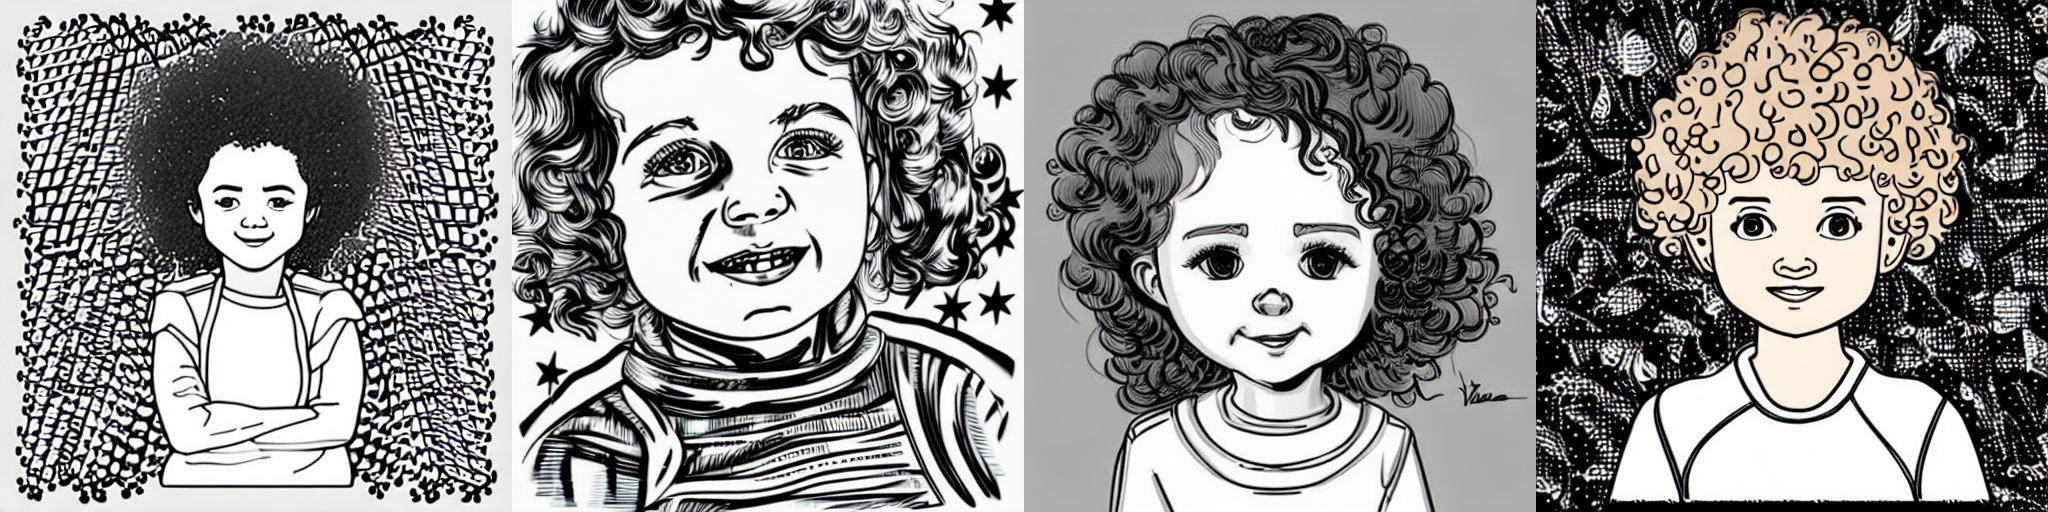
\includegraphics[width=1\linewidth]{figures/m9/en.png}\\
      
\includegraphics[width=0.95\linewidth]{figures/m9/zht.png}  & 
\includegraphics[width=1\linewidth]{figures/m9/zh.png}\\
      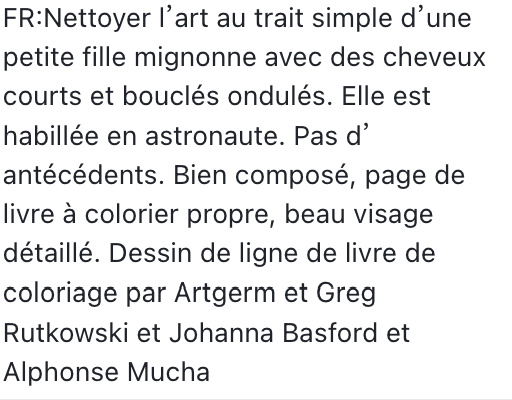
\includegraphics[width=0.95\linewidth]{figures/m9/frt.png}  & 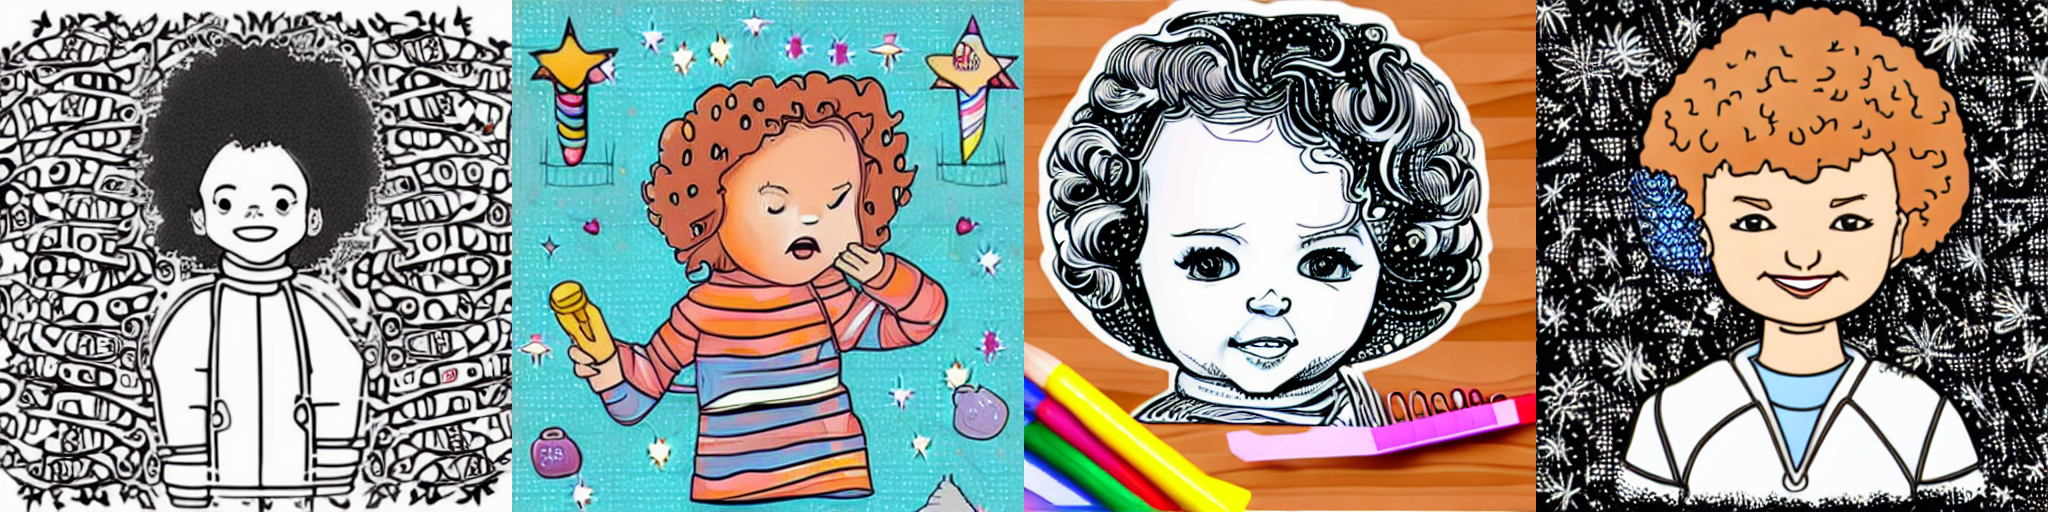
\includegraphics[width=1\linewidth]{figures/m9/fr.png}\\
      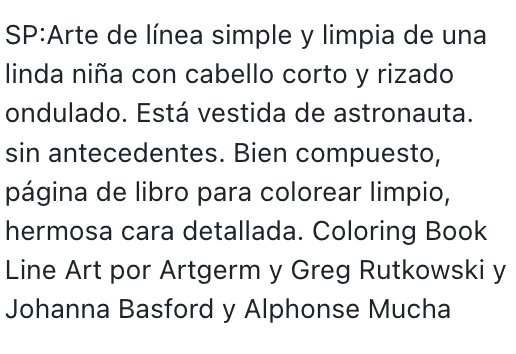
\includegraphics[width=0.95\linewidth]{figures/m9/spt.png}   & 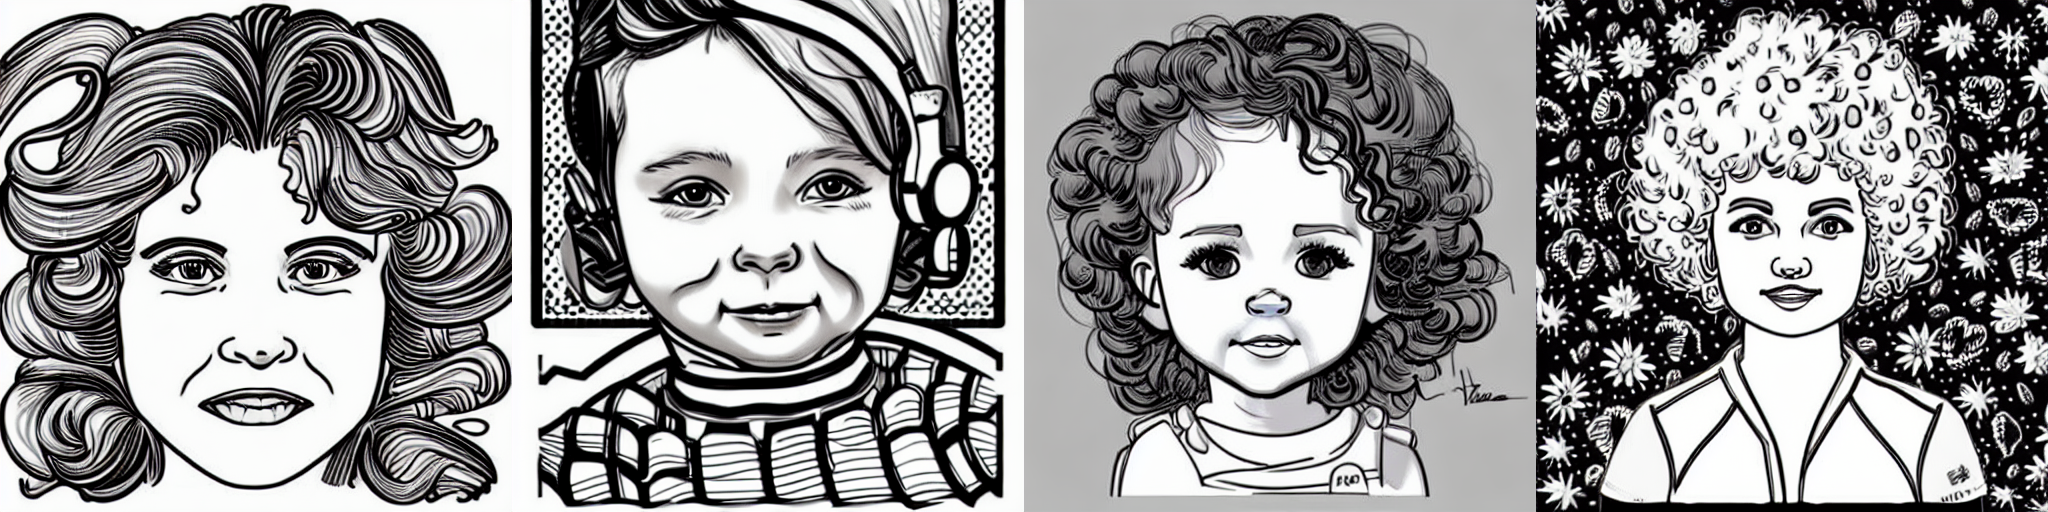
\includegraphics[width=1\linewidth]{figures/m9/sp.png}\\
       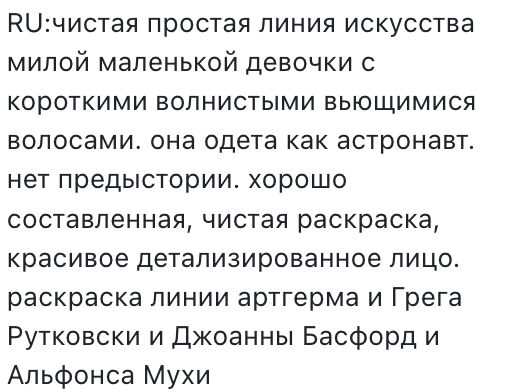
\includegraphics[width=0.95\linewidth]{figures/m9/rut.png}  & 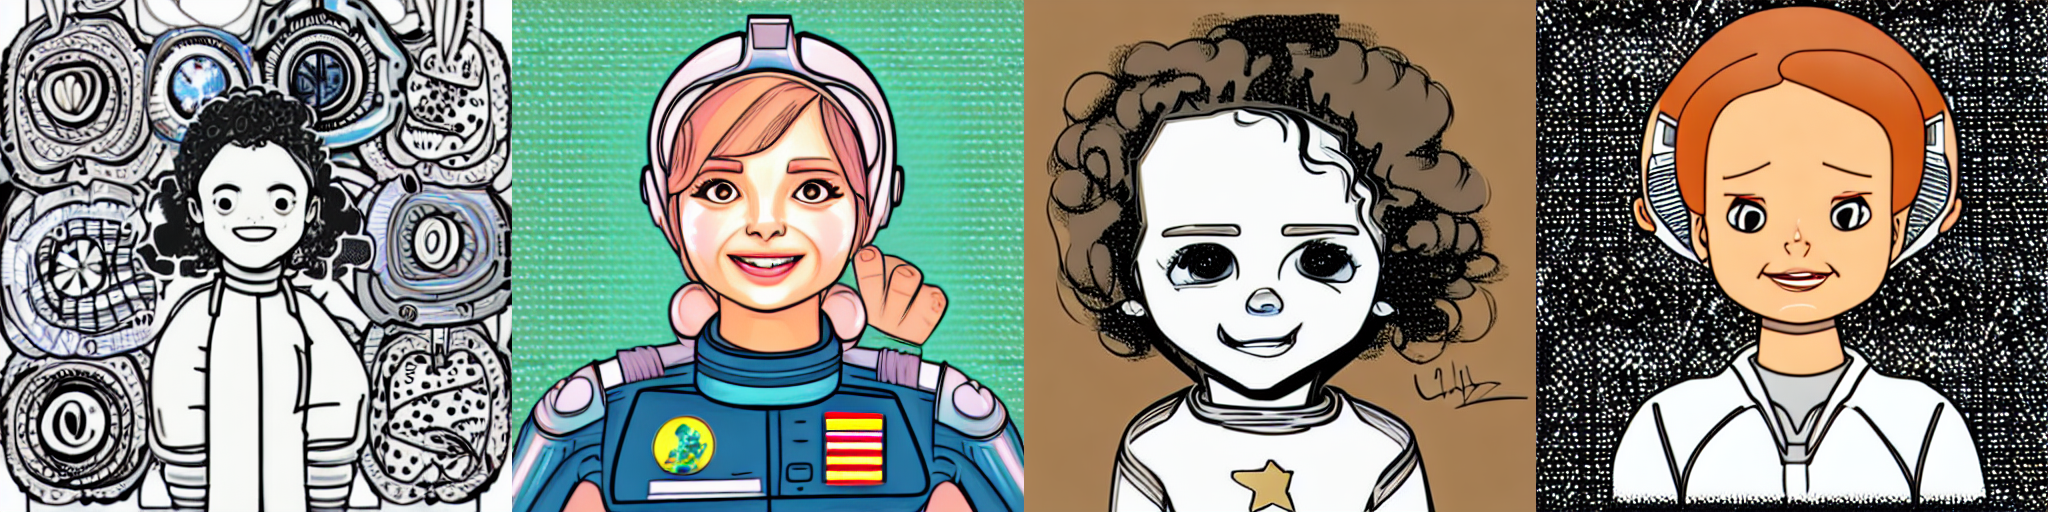
\includegraphics[width=1\linewidth]{figures/m9/ru.png}\\
        
\includegraphics[width=0.95\linewidth]{figures/m9/art.png}  & 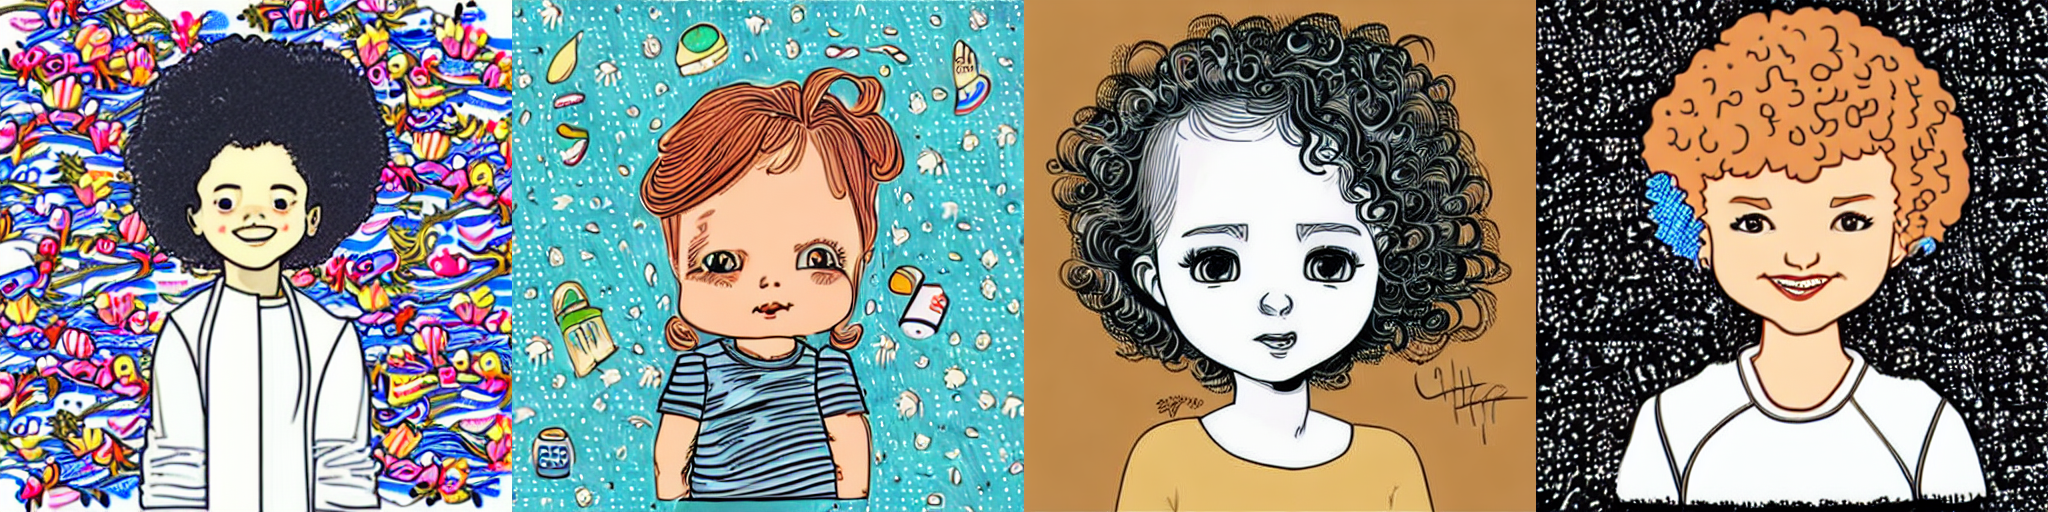
\includegraphics[width=1\linewidth]{figures/m9/ar.png}\\
         
\includegraphics[width=0.95\linewidth]{figures/m9/jat.png}   & 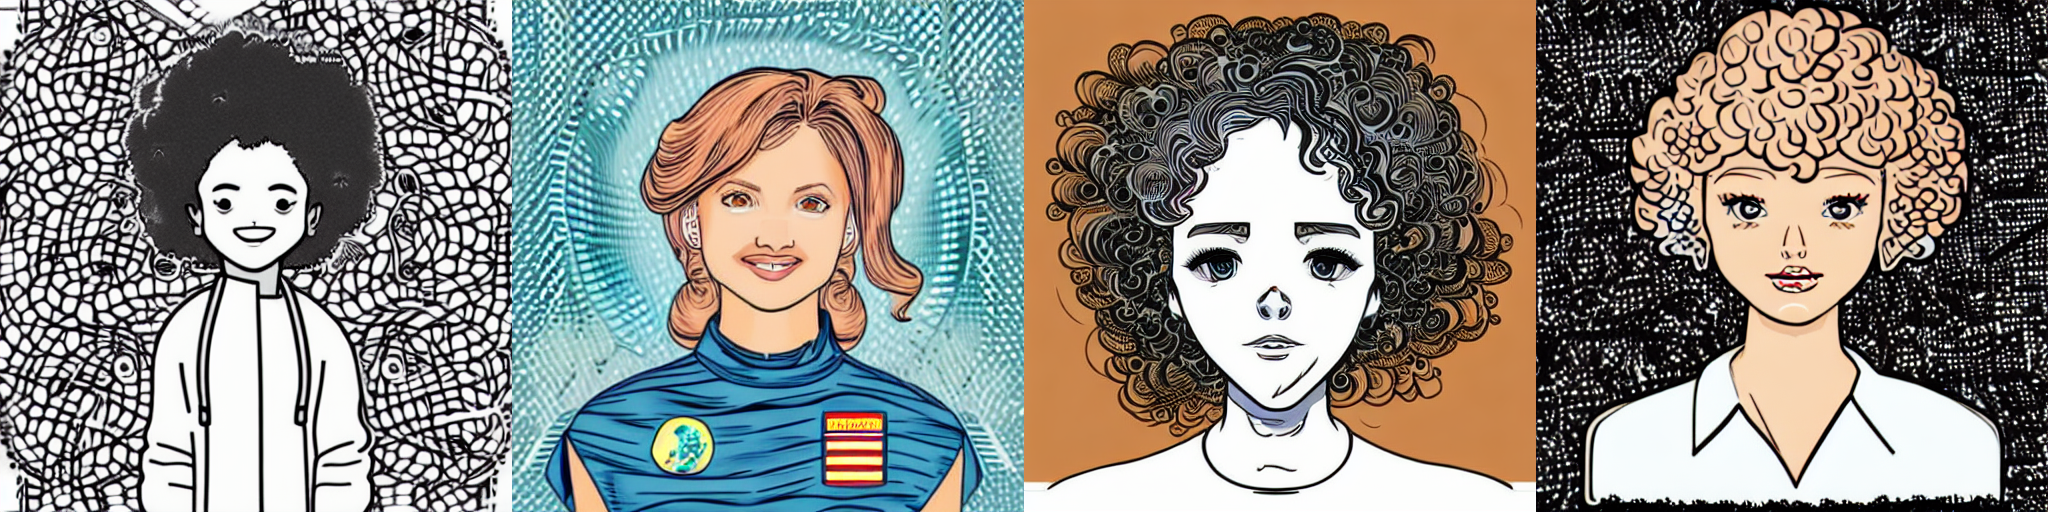
\includegraphics[width=1\linewidth]{figures/m9/ja.png}\\
          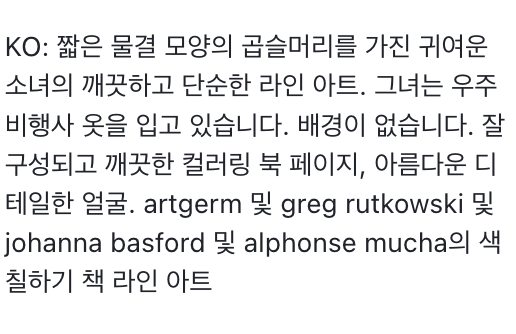
\includegraphics[width=0.95\linewidth]{figures/m9/kot.png}   & 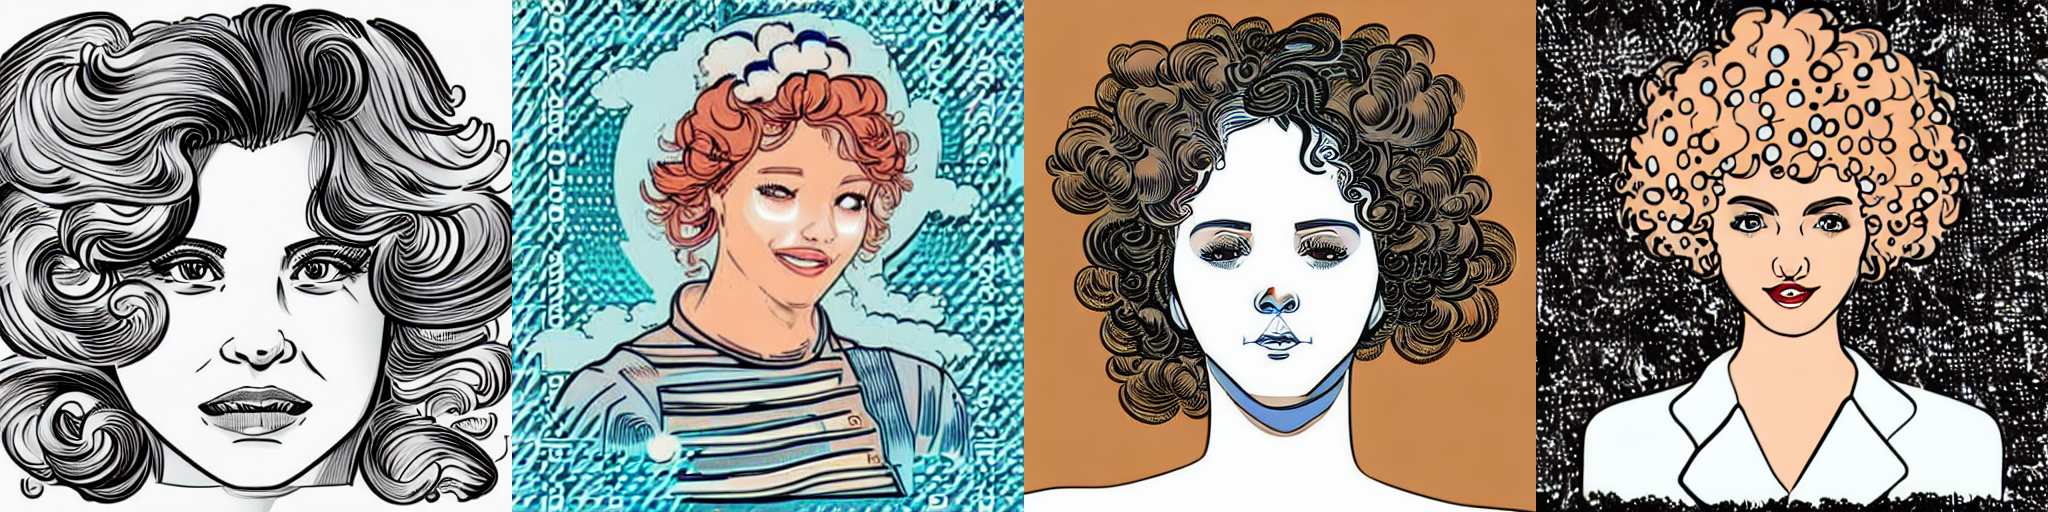
\includegraphics[width=1\linewidth]{figures/m9/ko.png}\\
           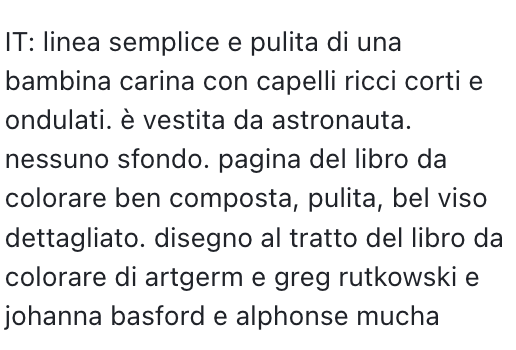
\includegraphics[width=0.95\linewidth]{figures/m9/itt.png}   & 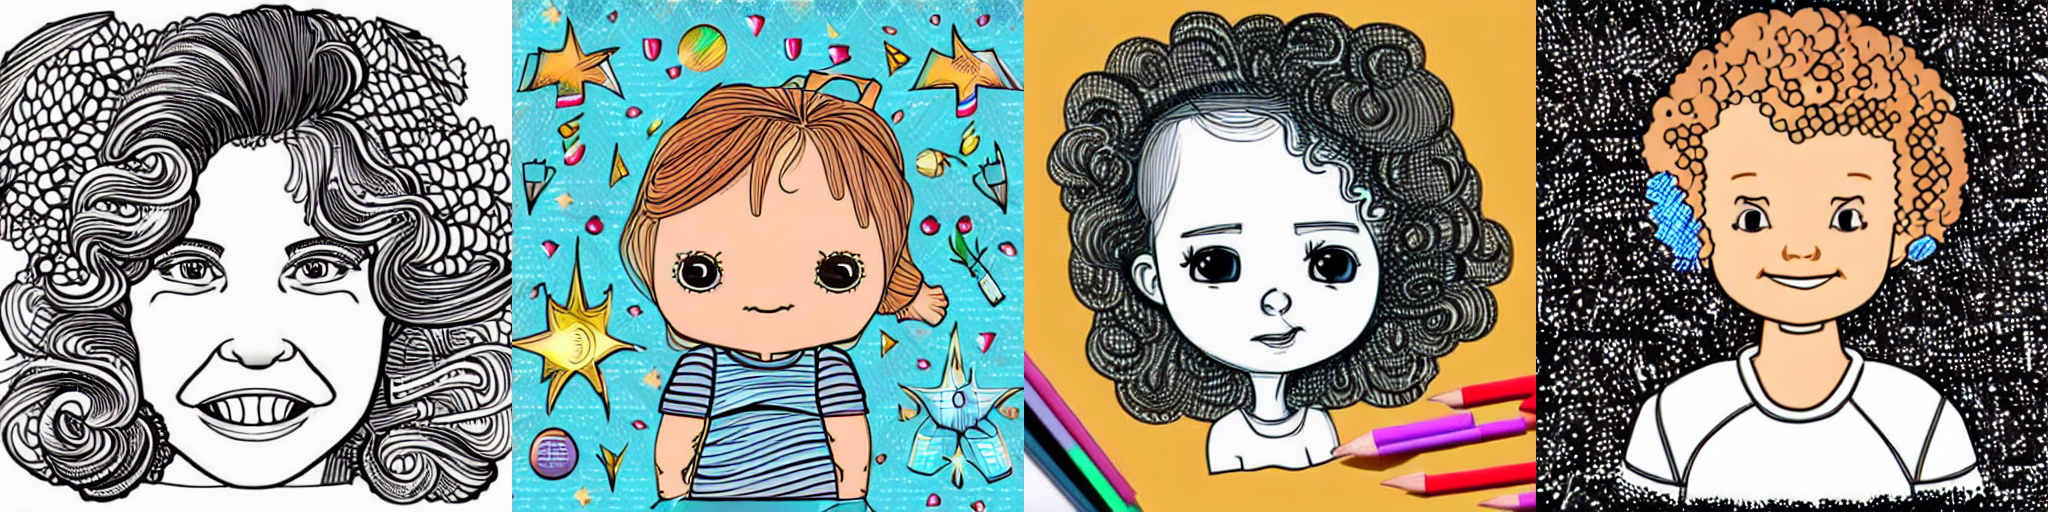
\includegraphics[width=1\linewidth]{figures/m9/it.png}\\\hline
    \end{tabular}
    \caption{The images generated by AltDiffusion$_{M9}$ with the same prompt translated to nine languages and a fixed seed.}
    \label{tab:m9}
\end{table*}
%\begin{figure}
%\centering
%\subfigure[Stable Diffusion] {
%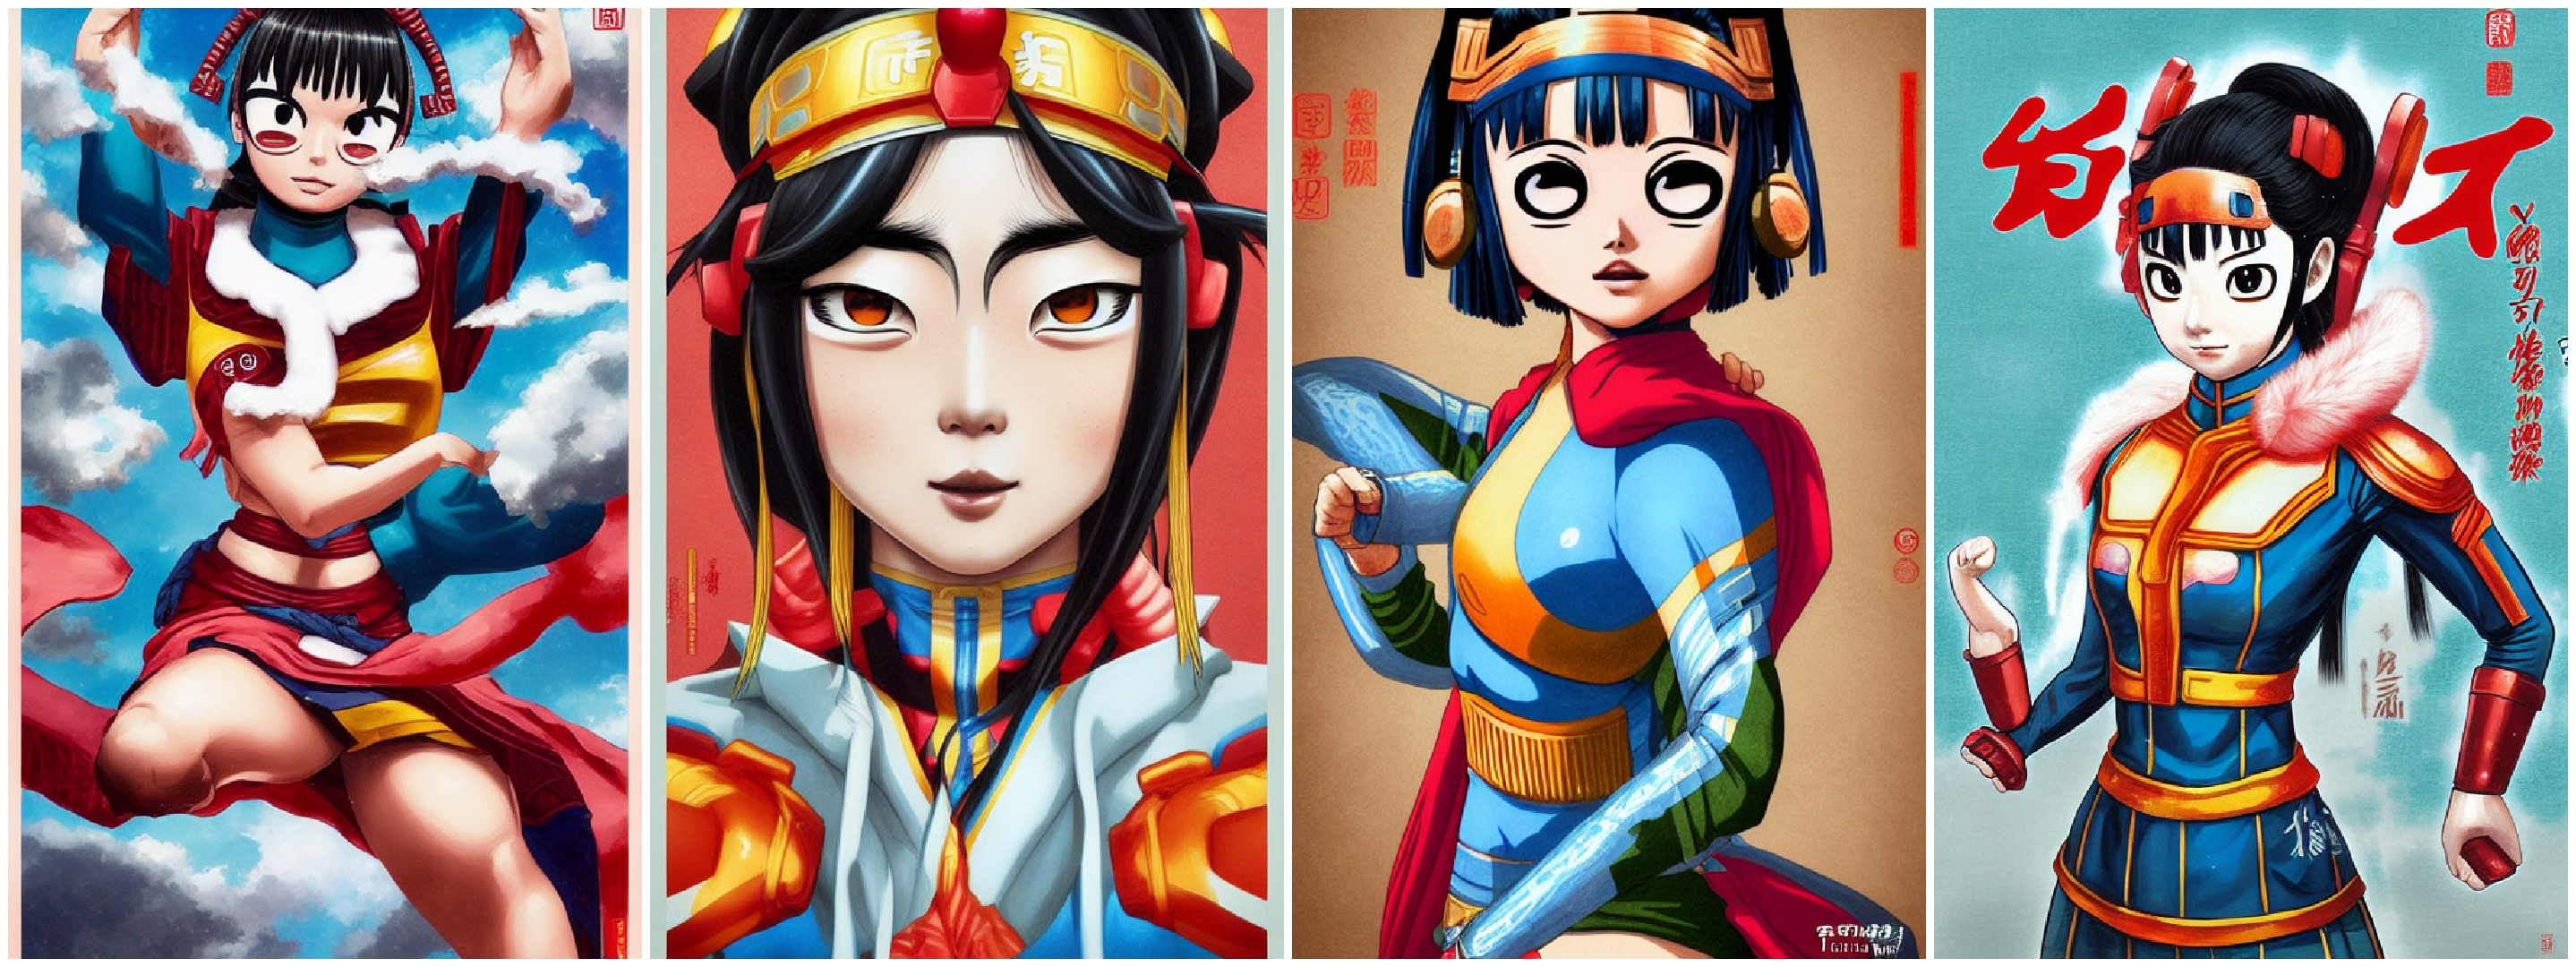
\includegraphics[width=0.45\textwidth]{figures/sd_better.jpg}
%}
%\subfigure[AltDiffusion] {
%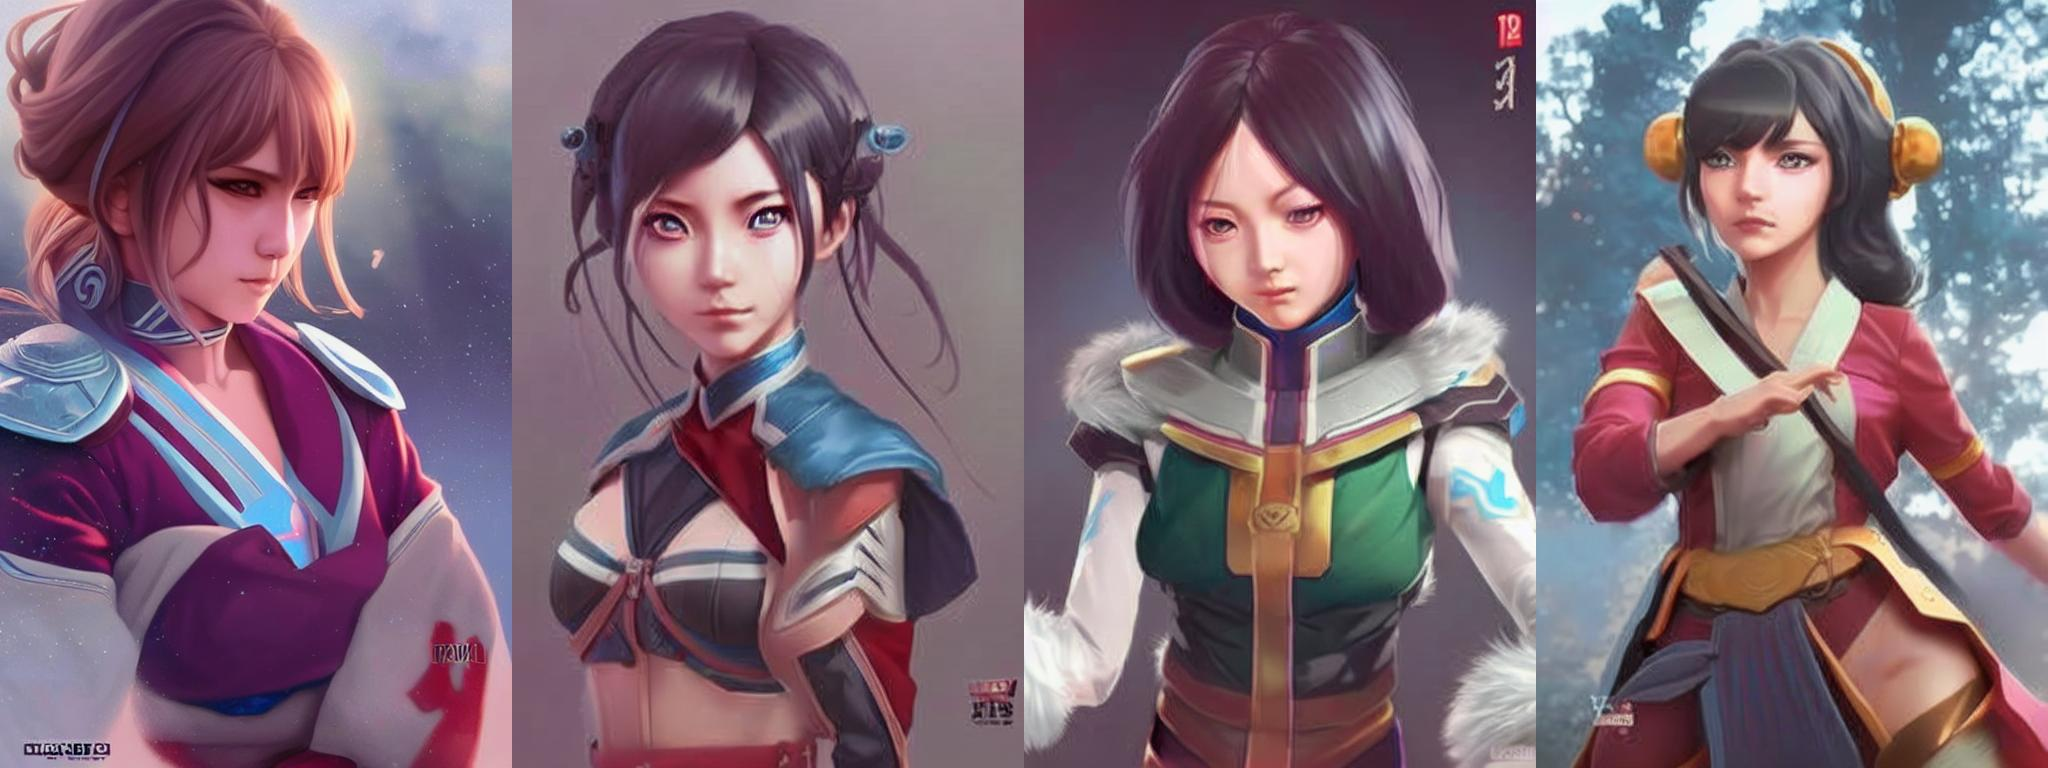
\includegraphics[width=0.45\textwidth]{figures/2_our_better.jpg}
%}
%\caption{Example of bilingual text-to-image generation. Text prompt: 
%\textit{"穿着唐朝服装, 唐朝, lofi Uraraka from My Hero Academia portrait, Pixar style, by Tristan Eaton Stanley Artgerm and Tom Bagshaw."}. The Chinese part in the prompt is translated to \textit{"Wearing Tang Dynasty clothing, Tang Dynasty"} for Stable Diffusion.
%}
%\label{fig:better_than_sd}
%\end{figure}


% \begin{table*}[bhtp]
% \centering
% \begin{tabular}{cc|ccccccc}\hline
% %Language & Dataset          & CLIP$_{\text{ViT-L}}$   &CN-CLIP$_\text{ViT-L}$  & AltCLIP$_\text{ViT-L}_{K}$ & AltCLIP^*$_\text{ViT-L}$ \\\hline
%  & Dataset          & CLIP & M-CLIP & M-CLIP$_{B}$ &CN-CLIP  &Wukong & AltCLIP$_{T}$ & AltCLIP  \\\hline
% \multirow{5}{*}{\rotatebox{90}{English}} &ImageNet    & \textbf{75.5} &52.3  &30  &32.5  &-  & 74.7           & 74.5      \\
% &ImageNet Sketch       & \textbf{59.6}  &44.2 &22.2   &30.7  &- & 59.2           & 58.7      \\
% &ImageNet-A             & \textbf{70.6} &59.1 &21.3 &29.8   &-  & 70.4           & 69.5      \\
% &ImageNet-R             & \textbf{87.9} &81.7  &48.3 &57.0  &-  & \textbf{87.9 }          & 87.2      \\
% &ImageNetV2             & \textbf{69.9} &47.3 &26.7  &28.6  &-  & 68.8           & 68.1      \\ \hline
% \multirow{5}{*}{\rotatebox{90}{Chinese}} & ImageNet   &  1.9  &43. &23.1 & 53.6    &58.2  &   58.2         &  \textbf{59.6}     \\
% & ImageNet Sketch                       &  1.9 &36.8 &17.2  &\textbf{47.3} & - &     44.5       &  46.5     \\
% &ImageNet-A                             & 6.0 &51.7 &16.4 & 43.1   &-  &     56.8       &   \textbf{58.5}    \\
% &ImageNet-R                              & 5.3 &68.7 &38.4 & 77.6  &-   &     78.0       &  \textbf{79.9 }    \\
% & ImageNetV2                             &  1.8 &40.1 &20.1 & 48.3 &-    &     48.1      &   \textbf{50.9}    \\ \hline
% \end{tabular}
% \caption{Comparison Results of our proposed model and sota CLIP models on image classification benchmarks, i.e. ImageNet and its variants. AltCLIP$_{T}$ and AltCLIP are the same to Figure 2. All image encoders used in these models are Vit-L for fair comparison. The metric reported is zero-shot classification accuracy.}
% \label{tab:imagenet}
% \end{table*}


% Please add the following required packages to your document preamble:
% \usepackage{multirow}




